\chapter{Линии и графы}

\setlength{\epigraphwidth}{.53\textwidth}
\epigraph{Человеческую душу радует небольшой беспорядок в своей геометрии.}{--- Луи де Берниер (1954---)}

%Человеку нравится неаккуратность в его геометрии

%Louis de Bernieres (2012). “Corelli's Mandolin: A Novel”, p.256, Vintage:

%The captain clicked his tongue disapprovingly, `Symmetry is only a property of dead things.
%Did you ever see a tree or a mountain that was symmetrical?
%It's fine for buildings, but if you ever see a symmetrical human face, you will have the impression that you ought to think it beautiful, but that in fact you find it cold.
%The human heart likes a little disorder in its geometry, Kyria Pelagia.
%Look at your face in a mirror, Signorina, and you will see that one eyebrow is a little higher than the other, that the set of the lid of your left eye is such that the eye is a fraction more open than the other.
%It is these things that make you both attractive and beautiful, whereas . . . otherwise you would be a statue. Symmetry is for God, not for us.'

%– Симметрия свойственна только мертвому. Вы когда-нибудь видели симметричные дерево или гору? Это хорошо для строений, а вот если бы вы увидели симметричноечеловеческое лицо, у вас бы сложилось впечатление, что его только полагается считать красивым, а на самом деле оно холодное. Человеческой душе нравится, чтобы в ее геометрии был небольшой беспорядок, кирья Пелагия. Посмотрите на себя в зеркало, синьорина, и вы увидите, что одна бровь у вас немного выше другой, что левое веко делает этот глаз чуточку шире. Но вы привлекательны и красивы, несмотря на... а иначе вы были бы статуей. Симметрия – для Господа, не для нас.

Мы спускаемся в одномерный мир --- к кривым, о которых вы знаете, и графам, о которых, возможно, не знаете.
Граф это просто набор точек, называемых вершинами, некоторые пары из которых образуют рёбра.
Часто вершины графа изображаются точками на плоскости, а его рёбра отрезками или кривыми, соединяющими одну свою вершину с другой.
При этом, если возможно обойтись без пересечений рёбер друг с другом, то граф называется \emph{планарным}.

\subsection*{Укрепление сетки}

У нас есть сетка размером $n \times n$ из стержней единичной длины, шарнирно соединённых в концах.
Вы можете укрепить некоторый набор $S$ маленьких квадратов диагональными скобками (длиной $\sqrt{2}$).

Какие наборы $S$ достаточны, для того чтобы сетка стала жёсткой на плоскости?

\begin{figure}[ht!]
\centering
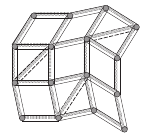
\includegraphics[scale=1]{pics/lattice1}
\caption{Недоукреплённая сетка.}
\label{pic:lattice1}
\end{figure}

На рис. \ref{pic:lattice1} показана недоукреплённая сетка $3 \times 3$.

\subsection*{Путешествие по острову}

Алоизий катается по острову на своём прекрасном автомобиле.
Известно, что на каждом перекрёстке острова сходится ровно три (двусторонние) улицы.
Алоизий придерживается следующего правила:
начав с какогот-то перекрёстка, он едет в произвольном направлении, на следующем перекрёстке он поворачивает направо, далее налево, затем направо, затем налево и так далее.

Докажите, что рано или поздно Алоизий вернётся на перекрёсток, с которого начал.

\parit{Замечание:} Граф, в котором к каждой вершине подходят ровно три ребра, называется \emph{кубическим}.
В нашем графе есть понятия \emph{право} или \emph{лево},
для этого достаточно чтобы граф был изображён на плоскости, с рёбрами (улицами) образованы кривыми.
При этом не обязательно требовать, чтобы граф был планарным;
можно разрешить мосты и туннели, то есть места, где ребра проходят один над другим.

\subsection*{Провода под Гудзоном}

Пятьдесят одинаковых проводов проходят под рекой Гудзон, все они выглядят одинаково.
Требуется определить все пары концов, принадлежащих одному проводу.
Для этого можно попарно замыкать любые провода на западном берегу и смотреть какие пары проводов на восточном образуют замкнутую цепь;
другими словами, вы можете определить, все пары проводов замкнутых на западном берегу.

Сколько потребуется поездок через Гудзон, чтобы выполнить эту задачу?

\subsection*{Жуки на четырёх прямых}

Даны четыре прямые на плоскости в общем положении (никакие две не параллельны, и никакие три не пересекаются в одной точке).
На каждой прямой жук-призрак ползёт с постоянной скоростью (возможно, разной для каждого жука).
Будучи призраками, при встрече жуки продолжают ползти сквозь друг друга.

Докажите, что если было пять из всех шести возможных встреч,
то была и шестая.

\medskip

Ну раз уж мы начали про жуков...

\subsection*{Пауки на кубе}

Три паука и муравей бегают по рёбрам куба.
Каждый паук бегает в три раза медленней муравья.
Докажите, что пауки смогут поймать муравья.

\medskip

Следующая головоломка подведёт нас к прекрасной теореме теории графов.

\subsection*{Вменяемые мыслители}

Граждане Перевёртовска каждую неделю встречаются и обсуждают городскую политику, в частности, стоит ли поддерживать строительство нового торгового центра.
Во время встреч каждый гражданин обсуждает этот вопрос со своими друзьями --- по какой-то причине их всегда нечётное число --- и на следующий день, при необходимости, меняет своё мнение относительно торгового центра так, чтобы оно совпадало с мнением большинства его друзей.

Докажите, что с какого-то момента, каждую вторую неделю у каждого будет то же самое мнение.

\parit{Замечание:}
Поскольку существует только конечное число наборов мнений ($2^n$, если в городе $n$ граждан), очевидно, что рано или поздно произойдёт зацикливание.
В данном случае утверждается, что период цикла должен быть $2$ (или $1$).
Почему такое может быть правдой?

\medskip

И под конец задача о ком-то, кто хочет остаться на своём графе.

\subsection*{Лемминг на шахматной доске}

На каждой клетке шахматной доски размера $n\times n$ есть стрелка, указывающая на одну из его восьми соседних клеток (или за пределы доски, если это крайняя клетка).
Однако направления стрелок в соседних клетках (включая диагональные) не могут различаться более чем на 45 градусов.

Лемминг начинает свой путь в центральном квадрате, следуя по стрелкам из квадрата в квадрат.
Придётся ли ему непременно упасть с доски?
